\section{Analysis of the dynamics -- equilibria and periodic orbits}

\begin{enumerate}
\item \textbf{Choosing parameters} Set parameters to physically sensible values. Choose $b$ according to optimality criterion \ref{pto_optimality_constraint}.

[Table of parameter values]

\item \textbf{Equilibria}

but first, let's study the equilibria

Define the \ac{bvp} that we are solving, explain why tauf = tau0 + 2pi

First return map converges, look at floquet exponents ?

\item \textbf{General behavior}

    hints at existence of two stable limit cycles

\item \textbf{Limit cycles}

\item \textbf{Algorithm for obtaining a limit cycle}

start form equilibrium, speed in correct direction, integrate until first return map converged.

\end{enumerate}

% TODO relevant? any implications?
All state and parameter values are normalized with unit length \(L\) the physical arm length, unit mass \(M\) the mass of the kite, and unit time \(T\) the wind speed at reference altitude over arm length ratio; therefore, \(a = m = v_{\mathrm{ref}} = 1\).

Let the state be \(vb x = (\vb q, \dq) = (\alpha, \tau, \dot \alpha, \dot \tau\). We are first interested in the steady states of the dynamical system, \emph{i.e.} static solutions with both zero velocity and acceleration. Therefore we are looking for solutions \(\vb q_0\) to

\begin{equation}
    \ddq(\vb q_0, \dq = 0) = 0 \in \R^2.
\end{equation}

In Figure~\ref{fig:equilibria-phase-space} we identify those solutions at the intersections of accelerations in \(\alpha\) and in \(\tau\): 4 null-clines for \(\ddot \tau\) that traverse the plot area horizontally and 2 for \(\ddot \alpha\) that traverse it vertically, therefore this system has \(4 \times 2 = 8\) steady states. We represent the configuration of the system at the steady states in Figure~\ref{fig:equilibria-eight-circle}.


\begin{figure}[thpb]
    \centering
    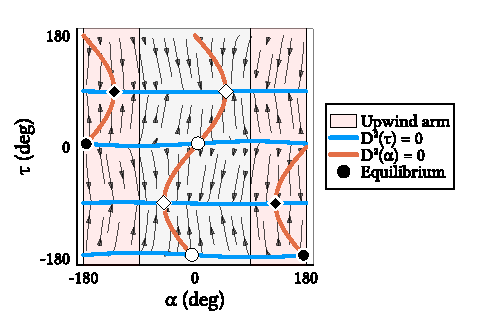
\includegraphics{figs/equilibria_phase_space}
    \caption{Zero velocity curves and equilibria of the dynamics.
    The black arrows represent the direction of the vector field $\ddq(\vq, \dq = 0)$, the green lines are the nullclines of $\ddot \alpha(\alpha, \tau)$, \emph{i.e.} the points $(\alpha, \tau)$ such that $\ddot \alpha(\alpha, \tau) = 0$, and the purple lines are the ones of $\ddot \tau(\alpha, \tau)$.
    At their intersections lie the equilibria of the system (all unstable), with color codes ranging from yellow to blue according to the highest real part of their eigenvalues.
    % TODO change graphical references in captions, also, says that max(Re(lambda i)) is approx 3 for circle and 12 for diamonds, for both colors
    The background is green when the arm points downwind and red when it points upwind.}
    \label{fig:equilibria-phase-space}
\end{figure}

\begin{figure}[thpb]
    \centering
    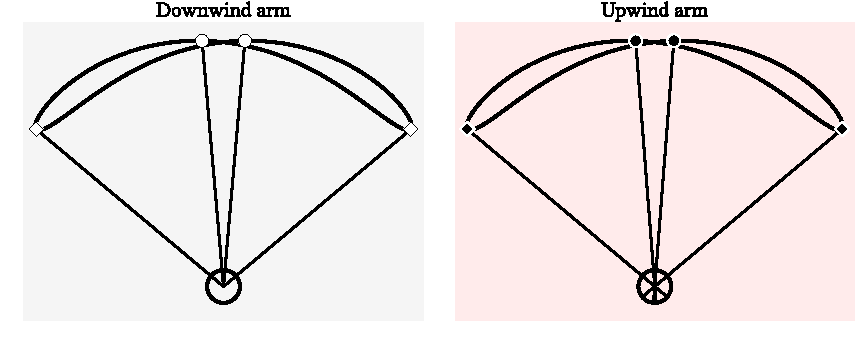
\includegraphics{figs/equilibria_eight_circle}
    % TODO For sale
    \caption{Configuration of the same equilibria in \emph{almost physical} top view of the system (the position of the kite is not adjusted according to the arm angle). We verified numerically that for all equilibria, the arm and the lines belong to the same vertical plane, \emph{i.e.} their projections in the $XY$ plane are aligned.}
    We find eight equilibria in total. They are unstable and we verify that for all of them, the lines and the arms are aligned when projected in the $x-y$ plane.
    % TODO move steady states descriptions here: one ss on the side (diamond), one near the center (circle), plus their symmetry through sigma (eq:symmetry), for both downwind and upwind arm.
    \label{fig:equilibria-eight-circle}
\end{figure}

Let us now look at dynamical solutions to this dynamical system. One such trajectory is a solution to

\begin{equation}
    \dot x = f(x)
\end{equation}
% TODO cite OrdinaryDiffEqVerner.jl
For integrating, we use the order-9 Verner method provided by OrdinaryDiffEqVerner.jl with absolute and relative integration tolerance of \(10^{-9}\) unless specified otherwise.

% TODO or adimensionalized?
Let \( x_0^{\pm} = (0, 0, 0, \pm 1)\) in normalized units. Time series for \(x_0^+\) exhibit a periodic orbit behavior.  

\begin{figure}[thpb]
    \centering
    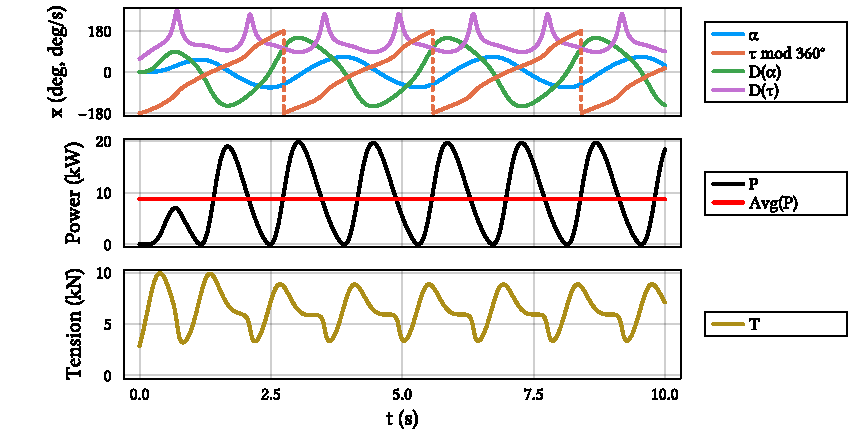
\includegraphics{figs/time_series_4D}
    % TODO give the initial state
    \caption{Time series of the state for a ten second integration. After a few seconds, the same pattern is repeated: this hints that our dynamical system exhibits a limit cycle.}
    \label{fig:timeseries}
\end{figure}



\begin{figure}[thpb]
    \centering
    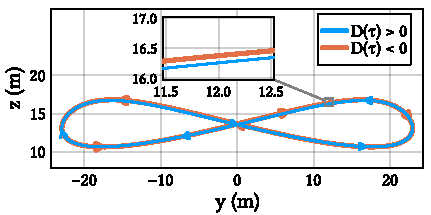
\includegraphics{figs/yz_limit_cycles}
    \caption{Projection of the kite trajectories onto the $YZ$ plane for the two limit cycles with opposite directions of motion (arrows indicate the direction of the kite motion). Zooming in on the trajectories shows that the two paths are distinct}
    \label{fig:yz_limit_cycle}
\end{figure}

Deflation algorithm for that set of parameters did not yield new limit cycles, on top of the two that are obtained with \(x_0^\pm\).


We define a sequence of states $(\vb x_i)_{i \geq 1}$ lying on a surface of section $\Sigma$, such that $\vb x_{i+1}$ is the first intersection between $\{\varphi^t(\vb x_i),\, t > 0\}$ and $\Sigma$, where $\varphi^t$ is the flow of ~\eqref{eq:eom}. Let
\begin{equation}
    \Sigma = \{\vb x \in T\mathbf{T}^2 \mid \tau(\vb x) = 0\}
\end{equation}
and $\Delta t(\vb x)$ be the time needed to achieve the first crossing of $\Sigma$ from state $\vb x$, namely:
\begin{equation}
    \Delta t(\vb x) = \min\{t > 0 \mid \varphi^t(\vb x) \in \Sigma\}.
\end{equation}
We then define the first recurrence map, or Poincaré map, as
\begin{equation}
    P : \vb x \in T\mathbf{T}^2 \mapsto \varphi^{\Delta t(\vb x)}(\vb x) \in \Sigma,
\end{equation}
and finally the desired sequence
\begin{equation}\begin{cases}
    \vb x_0 = P(\vb x^0) \\
    \vb x_{i+1} = P(\vb x_i).
\end{cases}\end{equation}

Since the trajectory starting at $\vb x^0$ approaches an attracting limit cycle, the limit of this sequence is defined and we plot the distance from $\vb x_i$ to $\vb x_\infty = \lim_{i \to \infty} \vb x_i$ in Figure~\ref{fig:convergence}.
The sequence converges exponentially, and in only $8$ iterations (seven revolutions over the lemniscate), we reach the precision limit of our ODE solver, with a distance of less than $10^{-12}$; in fact, we approximately gain $2$ digits of $\vb x_\infty$ after each revolution.
The points $\vb x_i$ are obtained using DifferentialEquations.jl's continuous callback feature, which saves the current state when a user defined function changes its sign, using the high-precision dense output from the ODE solver.

We confirm that there exist only two attracting limit cycles by sampling the state space with $(\alpha, \tau) \in \mathbf{T}^2$ and velocities $-M \leq \dot\alpha, \dot\tau \leq M$, and simulating the trajectory of each sampled point until convergence to a limit cycle with a \SI{1e-9} tolerance.
We choose $M = 10 \si{\radian\per\second}$ as upper bound; it corresponds to high arm and kite speeds which would be quickly damped by the generator and aerodynamic drag anyway.

\begin{figure}[thpb]
    \centering
    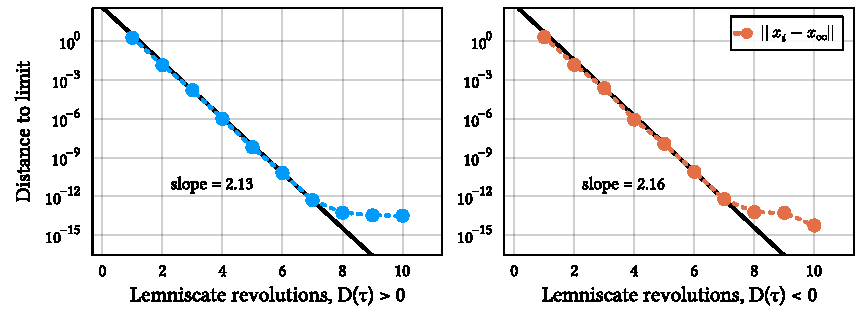
\includegraphics{figs/limit_cycle_convergence}
    \caption{Convergence toward the fixed point on the Poincaré map. The trajectory gets closer to the limit cycle as the number of lemniscate revolutions (a revolution is defined as a sweep over the interval $[0,2\pi]$ for the angle $\tau$) increases.
    The linear trend in log-linear plot indicates exponential convergence; after each revolution, the distance to the limit decreases by a factor of $10^{2.13}$ (\(\dot \tau > 0\)) or \(10^2.16\) (\(\dot \tau < 0\)), until it stalls near the tolerance of the integration scheme, set at \(10^{-13}\). The colored line is for \(\vb q_0 = (0, 0)\), perturbed trajectories are integrated from \(\vb q_0\) sampled in \([0, 2\pi]^2\).}
    \label{fig:limit_cycle_convergence}
\end{figure}
